\documentclass[10pt, a4paper]{article}
\usepackage[utf8]{inputenc}
\usepackage{listings}
\usepackage{hyperref}

\usepackage{fancyhdr}
\pagestyle{fancy}
\lhead{PERALE Thomas et RUSU George}
\rhead{INFO-F-203}

\usepackage{graphicx}
\usepackage{tikz}
\usepackage{color} or \usepackage{xcolor}

\lstset{ %
backgroundcolor=\color{white},   % choose the background color; you must add \usepackage{color} or \usepackage{xcolor}
basicstyle=\footnotesize,        % the size of the fonts that are used for the code
breakatwhitespace=false,         % sets if automatic breaks should only happen at whitespace
breaklines=true,                 % sets automatic line breaking
captionpos=b,                    % sets the caption-position to bottom
commentstyle=\color{mygreen},    % comment style
deletekeywords={\ldots},            % if you want to delete keywords from the given language
escapeinside={\%*}{*)},          % if you want to add LaTeX within your code
extendedchars=true,              % lets you use non-ASCII characters; for 8-bits encodings only, does not work with UTF-8
frame=single,                      % adds a frame around the code
keepspaces=true,                 % keeps spaces in text, useful for keeping indentation of code (possibly needs columns=flexible)
keywordstyle=\color{blue},       % keyword style
language=Octave,                 % the language of the code
otherkeywords={*,\ldots},           % if you want to add more keywords to the set
numbers=left,                    % where to put the line-numbers; possible values are (none, left, right)
numbersep=5pt,                   % how far the line-numbers are from the code
numberstyle=\tiny\color{mygray}, % the style that is used for the line-numbers
rulecolor=\color{black},         % if not set, the frame-color may be changed on line-breaks within not-black text (e.g.  comments (green here))
showspaces=false,                % show spaces everywhere adding particular underscores; it overrides 'showstringspaces'
showstringspaces=false,          % underline spaces within strings only
showtabs=false,                  % show tabs within strings adding particular underscores
stepnumber=2,                    % the step between two line-numbers.  If it's 1, each line will be numbered
stringstyle=\color{mymauve}, % string literal style
tabsize=2, % sets default tabsize to 2 spaces
title=\lst
}
\title{Rapport projet d'algorithmique 2}
\date{le 1 decembre 2015}

\begin{document}
\maketitle
\section{Introduction}
\parindent Dans un parking d'un centre commercial, Mademoiselle Goal d�sire sortir sa voiture le plus rapidement possible en ex�cutant le moins de man�uvre possible. Evidement le parking n'est pas vide, alors Mademoiselle Goal demande � ses amis les informaticien de l'aider. Notre but et de trouver sous forme de graphe (un noeud du graphe repr�sente une configuration du parking) le plus court chemin (le moins de manoeuvre possible) afin d'aider Mademoiselle Goal � rentrer chez elle.

\section{Cas de base}
\parindent Notre parking est un tableau n x n dans lequel plusieurs voiture s'y trouve. Parmi ces voitures, la voiture de Mlle, qui a notamment l'indicatif "G". Dans ce tableau, chaque cases peut contenir une voiture, g�n�ralement une voiture occupe deux cases. Il faut savoir qu'une voiture peut avancer ou reculer selon son orientation (verticale ou horizontale) jusqu'a la limite du tableau. L'unique voiture qui a le droit de sortir du tableau est bien �videment la voiture Goal.

\parindent Toutes les information n�cessaire � l'algorithme sont dans un fichier que notre programme recoit comme input gr�ce au argv.
\parindetn Voici un exemple de fichier:
    \lstinputlisting{../test/test1.txt}
    Celui ci nous renseigne sur:
    \begin{itemize}
        \item La taille du parking.
        \item La position de la sortie.
        \item L'emplacement des voitures dans ce parking.
    \end{itemize}
    Toute ces informations vont �tre pars� pour pouvoir cr�er un parking initial, qui sera notre
    cas de base � partir duquel il va falloir trouver le plus court chemin.\newline
    Conform�ment � l?�nonc�, l?algorithme ne fonctionnera que dans les cas suivant :
        \begin{itemize}
        \item Le fichier d'input est correctement �crit (pas d'erreur dans celui-ci), de la m�me mani�re que dans l'exemple.
        \item La voiture goal se d�place horizontalement (la sortie est sur la
            droite ou la gauche).
        \item Il n'y a pas de voiture de taille 1 (car impossible de savoir si
            elle se d�place horizontalement ou verticalement).
        \item Pas de parking de taille 0 (car pas possible d'y mettre une
            voiture goal).
    \end{itemize}

\section{Exemple d'utilisation.}
Exemple d'ex�cution en utilisant l'exemple au dessus.

\begin{lstlisting}
+---+---+---+---+---+
|     V2  V2        |
+   +   +   +   +   +
|         V3        |
+   +   +   +   +   +
| G   G   V3  V4
+   +   +   +   +   +
|             V4    |
+   +   +   +   +   +
|                   |
+---+---+---+---+---+

+---+---+---+---+---+
| V2  V2            |
+   +   +   +   +   +
|         V3        |
+   +   +   +   +   +
| G   G   V3  V4
+   +   +   +   +   +
|             V4    |
+   +   +   +   +   +
|                   |
+---+---+---+---+---+

+---+---+---+---+---+
| V2  V2  V3        |
+   +   +   +   +   +
|         V3        |
+   +   +   +   +   +
| G   G       V4
+   +   +   +   +   +
|             V4    |
+   +   +   +   +   +
|                   |
+---+---+---+---+---+

+---+---+---+---+---+
| V2  V2  V3        |
+   +   +   +   +   +
|         V3        |
+   +   +   +   +   +
|     G   G   V4
+   +   +   +   +   +
|             V4    |
+   +   +   +   +   +
|                   |
+---+---+---+---+---+

+---+---+---+---+---+
| V2  V2  V3        |
+   +   +   +   +   +
|         V3        |
+   +   +   +   +   +
|     G   G
+   +   +   +   +   +
|             V4    |
+   +   +   +   +   +
|             V4    |
+---+---+---+---+---+

+---+---+---+---+---+
| V2  V2  V3        |
+   +   +   +   +   +
|         V3        |
+   +   +   +   +   +
|         G   G
+   +   +   +   +   +
|             V4    |
+   +   +   +   +   +
|             V4    |
+---+---+---+---+---+

+---+---+---+---+---+
| V2  V2  V3        |
+   +   +   +   +   +
|         V3        |
+   +   +   +   +   +
|             G   G
+   +   +   +   +   +
|             V4    |
+   +   +   +   +   +
|             V4    |
+---+---+---+---+---+
\end{lstlisting}

\section{Description de la r�solution du probl�me.}
    Le probl�me va se faire en plusieurs �tapes:
    \begin{enumerate}
        \item Générer tout les configurations\footnote{Une configuration de
            parking est un parking avec les voitures à une certaine place.
            Quand on dit toutes les configurations possible on entend
            qu'à chaque fois qu'une voiture va bouger dans le parking on a une
            configuration différente.} de parking possible.
        \item Lors de cette génération, créer un graphe dans lequel chaques
            configurations nouvellement crée est lier à la configuration
            d'où elle vient.
        \item Une fois ces configurations générées, appliquer un algorithme de
            recherche du plus court chemin sur le graphe des configurations.
    \end{enumerate}

    Exemple\footnote{Les exemples sont créés à partir de
    http://analogbit.com/software/puzzletools/ .} de graphe associer aux
    configurations lors d'une génération non exhaustive (on abouti à deux
    situation gagnant2).

    % 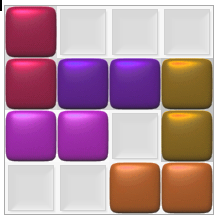
\includegraphics[scale=0.2]{gen0.png} \newline
    % \newpage
    \begin{tikzpicture}
        [scale=.8,auto=left,every node/.style={circle,fill=blue!20}]
        \node (n0) at (1, 10) {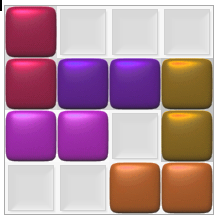
\includegraphics[scale=0.15]{gen0.png}};
        \node (n1) at (4, 10) {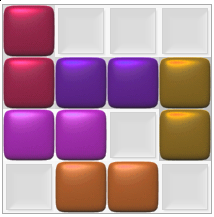
\includegraphics[scale=0.15]{gen1.png}};
        \node (n2) at (7, 10) {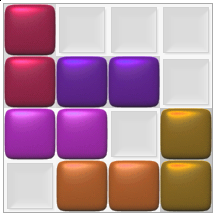
\includegraphics[scale=0.15]{gen2.png}};
        \node (n3) at (10, 10) {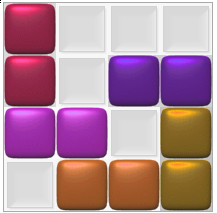
\includegraphics[scale=0.15]{gen3.png}};
        % Premier win

        %Autre situation à partir de n0
        \node (n4) at (1, 7) {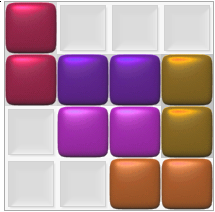
\includegraphics[scale=0.13]{gen4.png}};
        \node (n5) at (2, 5) {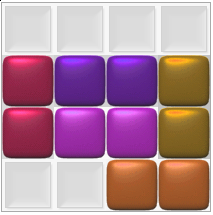
\includegraphics[scale=0.13]{gen5.png}};
        \node (n6) at (4, 4) {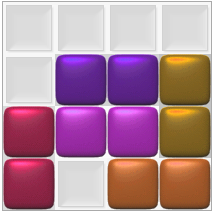
\includegraphics[scale=0.13]{gen6.png}};
        \node (n7) at (7, 4) {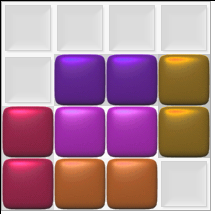
\includegraphics[scale=0.13]{gen7.png}};
        \node (n8) at (10, 4) {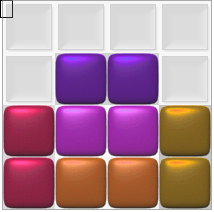
\includegraphics[scale=0.13]{gen8.png}};
        \node (n9) at (13, 4) {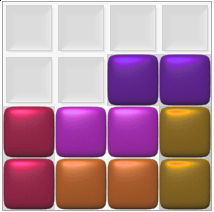
\includegraphics[scale=0.13]{gen9.png}};

        \node (n10) at (13, 4) {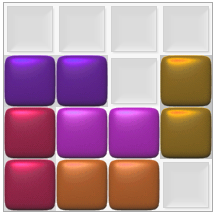
\includegraphics[scale=0.13]{gen10.png}};

        \foreach \from/\to in {n0/n1, n1/n2, n2/n3, n0/n4, n4/n5, n5/n6, n6/n7,
        n7/n8, n8/n9}
        \draw (\from) -- (\to);
    \end{tikzpicture}

\subsection{Génération des configurations.}
    Pour générer l'ensemble des solutions un algorithme de backtracking est
    utilisé, il fait avancer/reculer un maximum chaques voitures dans chaques
    configuration que cela va engendrer.
\subsection{Recherche du plus court chemin.}
    Pour trouver le plus court chemin parmis ceux générés. L'algorithme le plus
    évident pour effectuer un tel travail est l'algorithme de Dijkstra.
    Or ici nous avons un cas spécial de
    l'algorithme de Dijkstra car la distance entre chaques noeuds est de 1, là
    où l'algorithme de Dijkstra fait une recherche dans un graph où
    la distance entre deux noeuds est à chaques fois différente.
    Ainsi la \emph{min-priority queue} n'est pas nécessaire, une simple
    \emph{queue} peut être utilisé.
    L'algorithme ressemble donc à un parcour en largeur (\emph{breadth-first})
    qui s'arrête au premier parking \emph{gagnant} rencontré. \newline

    Exemple en mettant en évidence les profondeurs du parcour: \newline
    \begin{tikzpicture}
        [scale=.8,auto=left,every node/.style={circle,fill=blue!20}]
        \node (n0) at (1, 10) {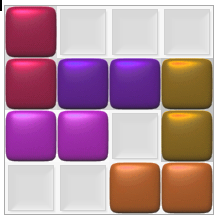
\includegraphics[scale=0.15]{gen0.png}};
        \node (n1) at (4, 10) {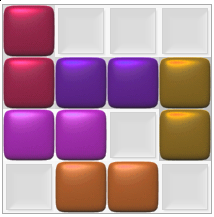
\includegraphics[scale=0.15]{gen1.png}};
        \node (n2) at (7, 10) {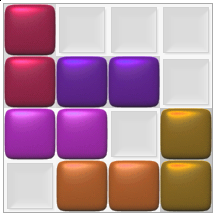
\includegraphics[scale=0.15]{gen2.png}};
        \node[color=green] (n3) at (10, 10) {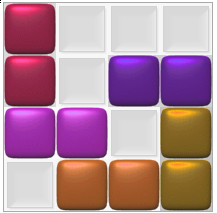
\includegraphics[scale=0.15]{gen3.png}};
        % Premier win

        %Autre situation à partir de n0
        \node (n4) at (1, 7) {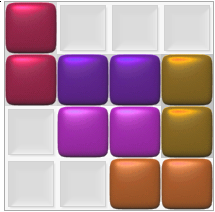
\includegraphics[scale=0.13]{gen4.png}};
        \node (n5) at (2, 5) {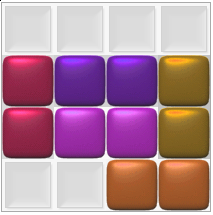
\includegraphics[scale=0.13]{gen5.png}};
        \node (n6) at (4, 4) {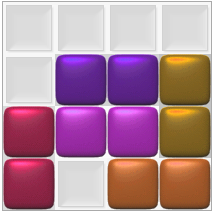
\includegraphics[scale=0.13]{gen6.png}};
        \node (n7) at (7, 4) {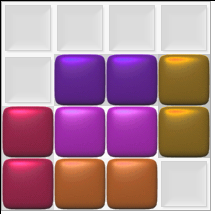
\includegraphics[scale=0.13]{gen7.png}};
        \node (n8) at (10, 4) {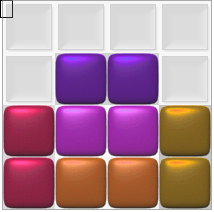
\includegraphics[scale=0.13]{gen8.png}};
        \node (n9) at (13, 4) {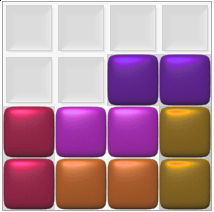
\includegraphics[scale=0.13]{gen9.png}};

        \node (n10) at (13, 4) {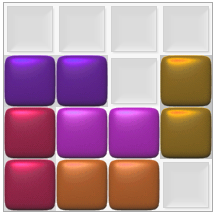
\includegraphics[scale=0.13]{gen10.png}};

        \foreach \from/\to in {n0/n1, n1/n2, n2/n3, n0/n4, n4/n5, n5/n6, n6/n7,
        n7/n8, n8/n9}
        \draw (\from) -- (\to);
        \draw[color=red]  (1, 8) to[out=10,in=-90] (3, 10);
        \draw[color=red]  (1, 6) to[out=0,in=-85] (5, 10);
        \draw[color=red]  (3, 5) to[out=90,in=-85] (8, 10);
        \draw[color=red] (6, 4) to[out=90,in=-85] (11, 10);
    \end{tikzpicture}



\section{Optimisation}
Une optimisation possible pour l'algorithme est de combiner la génération des
configurations avec la recherche du plus court chemins. Pour chaques noeuds que
l'on traite de notre queue (en commençant par le premier), on génère toutes les
configurations possible à partir de là, et ajoute chacune des nouvelles
configurations à cette queue pour être traité plus tard. En traitant les noeuds
de cette façon on fait aussi un parcour par couche (chaques couches génère la
suivante) mais on génère beaucoup moins de configuration comme on va arrêter
d'en générer dés qu'on tombe sur une configuration gagnante.

\newline

Exemple du traitement des parkings par couches (les chiffres correspondent au
moment où va être traité le parking):

\newline

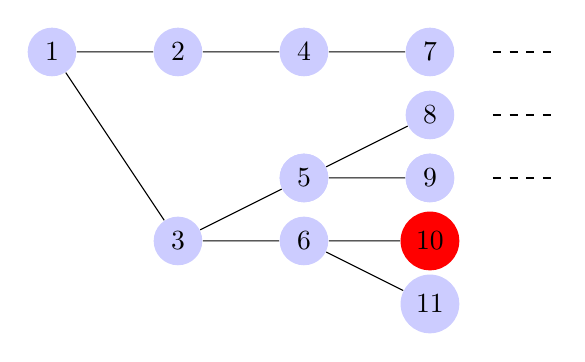
\begin{tikzpicture}
    [scale=.8,auto=left,every node/.style={circle,fill=blue!20}]
    \node (n0-0) at (1, 10) {1};
    \node (n0-1) at (3, 10) {2};
    \node (n0-2) at (5, 10) {4};
    \node (n0-3) at (7, 10) {7};
    % Premier win

    %Autre situation à partir de n0
    \node (n1-0) at (3, 7) {3};
    \node (n1-1) at (5, 7) {6};
    \node[fill=red] (n1-2) at (7, 7) {10};

    \node (n1-1-0) at (5, 8) {7};
    \node (n1-1-1) at (7, 8) {8};

    \node (n1-1-0-0) at (7, 9) {8};

    \node (n2-0) at (5, 8) {5};

    \node (n2-1) at (7, 8) {9};

    \node (n1-1-2) at (7, 6) {11};

    \foreach \from/\to in {n0-0/n0-1, n0-1/n0-2, n0-2/n0-3,
                           n0-0/n1-0,
                           n1-0/n1-1, n1-1/n1-2,
                           n1-0/n1-1-0, n1-1-0/n1-1-1,
                           n1-1/n1-1-2,
                           n1-1-0/n1-1-0-0}
    \draw (\from) -- (\to);
    \draw[dashed] (8, 10) -- (9, 10);
    \draw[dashed] (8, 9) -- (9, 9);
    \draw[dashed] (8, 8) -- (9, 8);
\end{tikzpicture}


\begin{thebibliography}
\bibitem{Rush Hour and Dijkstra's algorithm}
    Mark Stamp, Brad Engel McIntosh Ewekk, Victor Morrow,
    \emph{Rush Hour and Dijkstra's algorithm}
    http://www.cs.sjsu.edu/~stamp/cv/papers/rh.pdf

\end{thebibliography}

\end{document}
